\documentclass[spanish, fleqn]{article}
\usepackage[spanish]{babel}
\usepackage[utf8]{inputenc}
\usepackage{amsmath}
\usepackage{graphicx,float}
\usepackage{amsfonts,txfonts}
\usepackage{mathrsfs}
\usepackage[colorlinks, urlcolor=blue]{hyperref}
\usepackage{fourier}
\usepackage[top = 0.5cm, bottom = 1cm, left = 2cm, right = 2cm]{geometry}


\title{Presentación de Avance - Proyecto SWE \\ILI384: Taller de Modelos y Métodos Cuantitativos}
\author{Rodrigo Naranjo \and Martín Villanueva}
\date{11 de noviembre 2015}

\begin{document}
\maketitle

\thispagestyle{empty}


\section{Descripción del Problema}
El problema consiste en modelar el sistema de \textit{Shallow Water Equations} en $1D$ y $2D$, de tal modo
que se pueda determinar la evolución del sistema, dadas las ecuaciones diferenciales que modelan el problema,
las condiciones iniciales y las condiciones de borde. Las SWE corresponden a un caso particular de las ecuaciones
de Navier-Stokes, que se obtiene al hacer la suposición de que el fluido es incompresible, sin viscosidad y que la 
profundidad del agua es baja en relación al área en que se extiende. En el caso general (2D) las ecuaciones pueden 
escribirse como a continuación:
\begin{flalign}
 & \frac{\partial u}{\partial t} + u \frac{\partial u}{\partial x} + v \frac{\partial u}{\partial y} + g \frac{\partial h}{\partial x} = 0 \\
 & \frac{\partial v}{\partial t} + u \frac{\partial v}{\partial x} + v \frac{\partial v}{\partial y} + g \frac{\partial h}{\partial y} = 0 \\
 & \frac{\partial h}{\partial t} + \frac{\partial }{\partial x}(u(h-b)) + \frac{\partial }{\partial y}(v(h-b)) = 0 
\end{flalign}
donde las variables de interés (a modelar) son $h(x,y,t)$ (nivel de agua), $u(x,y,t)$ (componente de velocidad de una columna de
agua en $x$), $v(x,y,t)$ (componente de velocidad de una columna de agua en $y$).

\section{La Implementación}
Para la resolución del problema se plantea un enfoque del tipo partículas, donde la superficie del agua se modela por medio 
de un conjunto de partículas y por la forma en que se distribuyen. Para ser más precisos, cada una de las variables de interés 
($h$, $u$ y $v$) se aproximan como una combinación lineal de funciones $RBF$. Para $h$, por ejemplo, se tiene:

$$h(x,y,t) = \sum_{i=0}^{N} \gamma_i(t)\Phi(||\mathbf{x}-\boldsymbol{\xi}_i(t)||, \epsilon_i(t))$$
 
donde la función RBF a ocupar es de preferencia una función de soporte compacto, de modo que se acote el radio de influencia 
de cada función. 

Lo que se quiere lograr sigue el enfoque \textit{Evolutive RBF}, donde se obtienen ecuaciones de evolución (ODE's) para los 
parámetros dependientes del tiempo en cada RBF ($\gamma(t)$, $\boldsymbol{\xi}_i(t)$ y $\epsilon_i(t)$). En dicho caso, para 
obtener el estado del sistema en un $t+\triangle t$, sería tan sólo computar las ecuaciones de evolución para cada RBF 
(de cada variable) y luego sumar los resultados respectivos en el espacio.

Inicialmente, se propone resolver las \emph{Burger's Equations} en 1D sin viscosidad, definidas por:
\begin{flalign}
  \frac{\partial u}{\partial t} + u\frac{\partial u}{\partial x} = 0
\end{flalign}
Se puede observar que esta es una versión simplificada de las SWE, en las cuales no se considera la ecuación de continuidad.

El siguiente paso, consiste en resolver las SWE en 1D (solo se considerará el movimiento en el eje X), a modo de obtener una 
aproximación para estudiar el comportamiento de las ecuaciones antes de avanzar al problema en 2D.

Finalmente, se implementarán las SWE en 2D.

\section{Dificultades}
Se presentan aquí algunas de las dificultades que se conocen, y otras que eventualmente podrían aparecer en la implementación 
del proyecto.
\begin{itemize}
	\item La batimetría $b(x,y,t)$ es, en general, una función discontinua (o que se conoce parcialmente), y por lo tanto 
	debe hallarse una manera de aproximar su derivada.
	\item En simulaciones ocupando otros métodos (SPH \textit{Smoothed Particle Hidrodynamics}) se ha notado que no tomar 
	en cuenta la viscosidad, puede llevar a problemas de estabilidad numérica en las simulaciones.
	\item Probablemente en las simulaciones sea necesario ocupar una gran cantidad de partículas para modelar la superficie
	del agua, lo cual lleva a una gran cantidad de computación para determinar los estados siguientes del sistema. Por ello,
	quizas sea necesario paralelizar la ejecución, o buscar métodos más eficientes de computación (FMM Fast Multipole 
	Method).
\end{itemize}                                                                                                                                                                                                                                                                                                                                                                                                     

\section{Desarrollo}
  \subsection{Burger's Equation}
    Para realizar una prueba preliminar antes de modelar las SWE, se procedió a resolver la Burger's Equation, una ecuación que 
    permite modelar de manera simplificada el comportamiento de un fluido incompresible.
    
    Para realizar esto, se procedió a modelar el comportamiento de la función $u(x,t)$ mediante el uso de 
    \textit{Evolutive RBF} de la siguiente forma:
    \begin{align*}
      \Phi_u(x,t) = \sum_i \gamma_i(t)\phi_i(x-\xi(t),\epsilon_i)
    \end{align*}
    Donde $\Phi_u$ es una aproximación de $u(x,t)$ mediante la suma de funciones \textit{RBF}. Para casos de prueba iniciales, 
    se usará la función $\phi$ definida como:
    \begin{align*}
      \phi(x,\epsilon) = e^{-(\epsilon x)^2}
    \end{align*}
    Donde $\epsilon$ corresponde al inverso del \textit{shape parameter} de la \textit{RBF}. En el futuro, se pretende 
    reemplazar esta función por funciones de soporte compacto, con el fin de generar sistemas \textit{sparse}.
    
    Se realizó un experimento modelando el comportamiento de la ecuación para el estado inicial:
    \begin{equation*}
      u(x) = I_{x \in [7,12]}\frac{(7-x)(x-12)}{12}
    \end{equation*} \\
    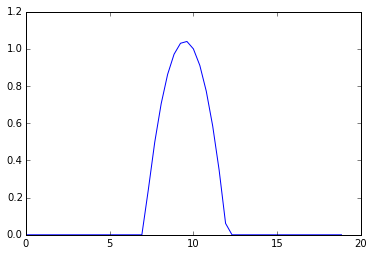
\includegraphics[scale=0.6]{initialu.png} \\
    La aproximación inicial utilizando \textit{RBF} fue la siguiente: \\
    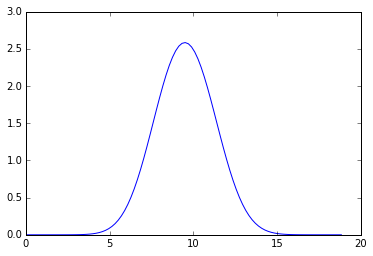
\includegraphics[scale=0.6]{rbfapp.png} \\
    Resolviendo el sistema de ecuaciones, se hallaron las ecuaciones de evolución de los parámetros de la \textit{RBF} de la 
    forma:
    \begin{align*}
      \gamma'(t) &= 0 \\
      \epsilon'(t) &= 0 \\
      \xi'(t) &= u
    \end{align*}
    Estas ecuaciones indican que las \textit{RBF} mantendrán su forma ($\gamma'(t) = \epsilon'(t) = 0$). Los cambios de forma
    en el fluido ocurrirán debido a la superposición de las \textit{RBF} a medida que estas se muevan acorde a la última 
    ecuación.
    
    Algunos resultados obtenidos para la evolución de la ecuación en el tiempo son los siguientes: \\
    \begin{figure}[H]
      \centering
      \begin{minipage}{.5\textwidth}
        \centering
        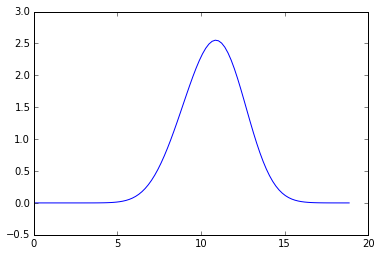
\includegraphics[scale=0.6]{t1000.png}
      \end{minipage}%
      \begin{minipage}{.5\textwidth}
        \centering
        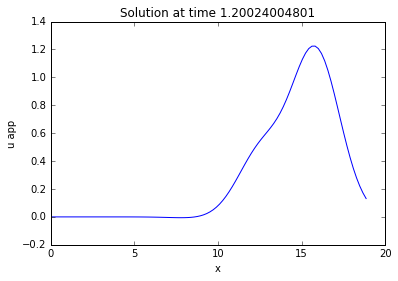
\includegraphics[scale=0.6]{t2000.png}
      \end{minipage}
    \end{figure}
    \begin{figure}[H]
      \centering
      \begin{minipage}{.5\textwidth}
        \centering
        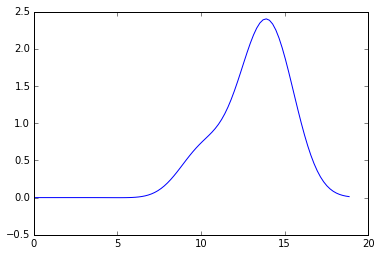
\includegraphics[scale=0.6]{t3000.png}
      \end{minipage}%
      \begin{minipage}{.5\textwidth}
        \centering
        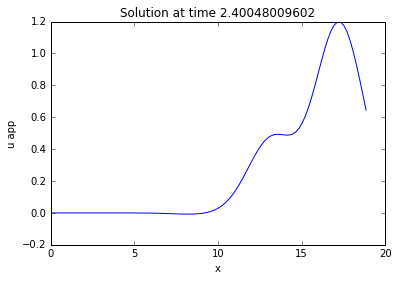
\includegraphics[scale=0.6]{t4000.png}
      \end{minipage}
    \end{figure}
    \begin{figure}[H]
      \centering
      \begin{minipage}{.5\textwidth}
        \centering
        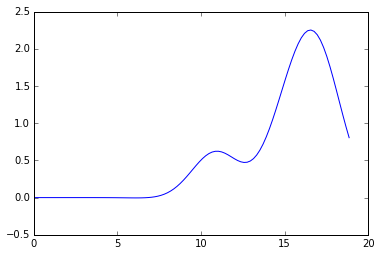
\includegraphics[scale=0.6]{t5000.png}
      \end{minipage}%
    \end{figure}
    Como se puede observar, el comportamiento modelado por la \textit{Burger's Equation} es bastante simple, consistiendo en un
    movimiento de la perturbación inicial $u(x,0)$ acorde a su posición anterior. Algunos de los detalles que pudieron 
    observarse en la simulación son la aparición de una perturbación más pequeña que parece moverse a menor velocidad que el
    resto del sistema.
    
\vfill\hfill RN/MV/\LaTeXe
\end{document}